%--------------------
% Packages
% -------------------
\documentclass[11pt,a4paper]{article}
\usepackage[utf8x]{inputenc}
\usepackage[T1]{fontenc}
%\usepackage{gentium}
\usepackage{mathptmx} % Use Times Font


\usepackage[pdftex]{graphicx} % Required for including pictures
% \usepackage[swedish]{babel} % Swedish translations
\usepackage[pdftex,linkcolor=black,pdfborder={0 0 0}]{hyperref} % Format links for pdf
\usepackage{calc} % To reset the counter in the document after title page
\usepackage{enumitem} % Includes lists

\frenchspacing % No double spacing between sentences
\linespread{1.2} % Set linespace
\usepackage[a4paper, lmargin=0.1666\paperwidth, rmargin=0.1666\paperwidth, tmargin=0.1111\paperheight, bmargin=0.1111\paperheight]{geometry} %margins
%\usepackage{parskip}

\usepackage[all]{nowidow} % Tries to remove widows
\usepackage[protrusion=true,expansion=true]{microtype} % Improves typography, load after fontpackage is selected

% \usepackage{lipsum} % Used for inserting dummy 'Lorem ipsum' text into the template
\usepackage{amsmath}

%-----------------------
% Set pdf information and add title, fill in the fields
%-----------------------
\hypersetup{ 	
pdfsubject = {},
pdftitle = {},
pdfauthor = {}
}

%-----------------------
% Begin document
%-----------------------
\begin{document} %All text i dokumentet hamnar mellan dessa taggar, allt ovanför är formatering av dokumentet
\title{Bayesian Neural Networks}
\date{}
\author{Purna Vindhya, Kota}
\maketitle

% Bayesian Neural Networks



\section{Introduction}

Given some input–output (x → y) data, we wish wishes to learn a regressor $f(\cdot)$ for prediction $y^{\star} = f(x^{\star})$ given a new input $x^{\star}$. Neural networks are a type of regressor that consists of multiple layers of simple nonlinear functions, parameterized by a set of weights (and biases), $\omega$. Training the neural networks refers to calibrating the value of these weights using the available training data $\mathcal{D} = \{x,y\}$. \\
To represent the aleatoric uncertainties, adopt a probability model over the data, say normal distribution:

\begin{equation}
    p(y|x, \omega) = \mathcal{N}(y; NN_{\omega}(x), \sigma_n ^2) \label{eq:1}
\end{equation}
In this study, the aim is to quantify the epistemic uncertainties, thus the variation of measurement noise $\sigma_n ^2$ can be assumed apriori. Assuming training data points are i.i.d., the likelihood over the whole dataset $\mathcal{D}$ is computed as:

\begin{equation}
    p(\mathcal{D}|\omega) = \Pi_{i=1}^{n} \mathcal{N}(y_i ; NN_{\omega}(\omega), \sigma_n ^2)
\end{equation}
Epistemic uncertainties are quantified by learning a probability model over the parameters of the model $\omega$. In a Bayesian setting, the prior $p_0(\omega)$ can be assumed apriori. With the data, the posterior on the weights is updated as:

\begin{equation}
    p(\omega|\mathcal{D}) = \frac{ p(\mathcal{D}|\omega) p_0(\omega) }{p(\mathcal{D})}
\end{equation}
Therefore, during prediction, given a new input $x^{\star}$,
\begin{equation}
    p(y^{\star}| x^{\star}, \mathcal{D}) = \int p(y^{\star}| x^{\star}, \omega) p(\omega|\mathcal{D})d\omega
\end{equation}
The epistemic uncertainty can be quantified as the variance of $y^{\star}| x^{\star}, \mathcal{D}$. In a deterministic setting, the optimum weights $\omega$ can be found by:
\begin{equation}
    \omega^{opt} = argmx_{\omega} \log( p(\mathcal{D}|\omega) p_0(\omega) )
\end{equation}
and is equivalent to the standard training procedures of a neural network. To accurately quantify the epistemic uncertainties within the NN, the full posterior pdf must be inferred. 
A Bayesian Neural Network (BNN) is a probabilistic model that allows us to estimate uncertainty in predictions by representing the weights and biases of the network as probability distributions rather than fixed values. This allows us to incorporate prior knowledge about the weights and biases into the model, and update our beliefs about them as we observe data. BNNs are a handy tool to quantify the uncertainty over the posterior. Moreover, they provide estimates around predictions without the need for separate training, validation, and test data sets. 
To estimate the (intractable) posterior distribution $p(\omega|\mathcal{D})$, we can use
\begin{itemize}
    \item Variational methods
    \item Markov Chain Monte Carlo sampling
\end{itemize}




\section{Models}
\subsection{Stochastic Variational Inference}

The normalized posterior probability density $p(\omega|\mathcal{D})$ is intractable, so we approximate it with a tractable parametrized density $q_{\phi}(\omega)$ from a family of probability densities $\mathcal{Q}$. The variational parameters are denoted by $\phi$. The goal is to find the variational probability density that best approximates the posterior by minimizing the KL divergence

\begin{math}
    KL(q_{\phi}(\omega)||p(\omega|\mathcal{D}))
\end{math} \\
with respect to the variational parameters $\phi$. However, directly minimizing the KL divergence is not tractable because we assume that the posterior density is intractable. To solve this, we use Bayes theorem to obtain

\begin{equation}
    \log p(\mathcal{D}|\omega) = KL\big(q_{\phi}(\omega)||p(\omega|\mathcal{D})\big) + ELBO(q_{\phi}(\omega))
\end{equation}
\begin{equation}
        \text{ELBO}(q_{\phi}(\omega)) = \mathbb{E}_{\omega \sim q_{\phi}(\omega)}[ p(y|x,\omega)] - \text{KL}(q_{\phi}(\omega) || p(\omega))
\end{equation}
By maximizing the ELBO, we indirectly minimize the KL divergence between the variational probability density and the posterior density. Therefore, the ELBO loss function:
\begin{equation}
    \mathcal{L} = \text{KL}(q_{\phi}(\omega) || p(\omega) ) - \mathbb{E}_{\omega \sim q_{\phi}(\omega)}[\log p(\mathcal{D},\omega) ]
\end{equation}

For the full-covariance Gaussian approximate posterior, the model weights for each layer $\omega_i$ are distributed according to the multivariate Gaussian distribution $\mathcal{N}(\bm{\mu}_i, \bm{\Sigma}_i)$. The mean-field approximation restricts $\bm{\Sigma}_i$ to be a diagonal covariance matrix, or equivalently assumes that the probability distribution can be expressed as a product of individual weight distributions:
\begin{equation}
    \mathcal{N}(\bm{\mu}_i, \bm{\Sigma}_i) = \Pi_j \mathcal{N}(\mu_{ij}, \sigma_{ij})
\end{equation}

The mean-field approximation greatly reduces the computational cost of both forward and backwards propagation, and reduces the number of parameters required to store the model from order $n^2$ in the number of weights to order $n$.

The \textit{Stochastic Variational Inference (SVI)} is a stochastic optimization algorithm for mean-field variational inference. The algorithm approximates the posterior distribution of a probabilistic model with hidden variables. SVI by using a normal probability density with a diagonal covariance matrix. The algorithm uses stochastic gradient ascent to optimize the ELBO with respect to the global variational parameters. The SVI algorithm is explained in detail in \cite{hoffman}

\subsubsection{Problem Description}
The data that we are trying to fit to the BNN is:
\begin{equation}
    y = x + 0.3 \sin(2 \pi x) + 0.3 \sin(4 \pi x)
\end{equation}
where, 
\begin{math}
    x = [-0.5,1.5] + \epsilon \text{ and, }
    \epsilon \sim \mathcal{N}(0,0.02)
\end{math}

\begin{figure}[h!]
    \centering
    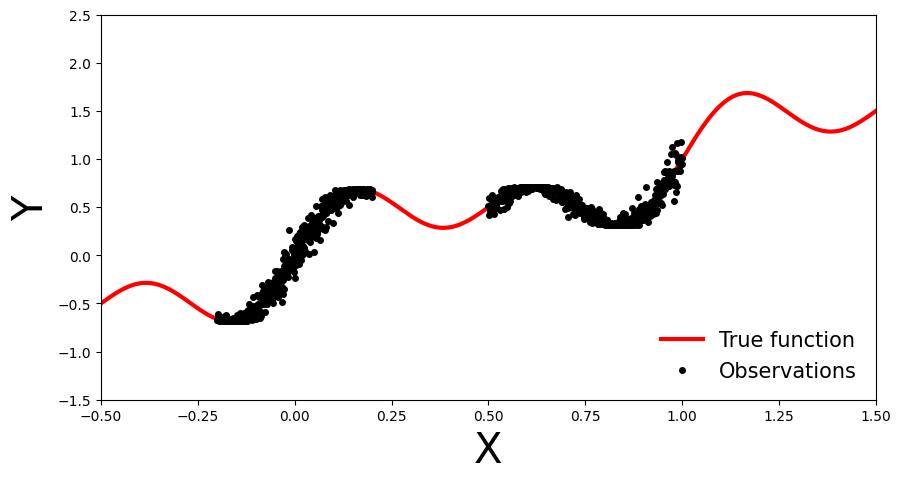
\includegraphics[scale=0.5]{original data.png}
    \caption{True function and data points}
    \label{fig:train data}
\end{figure}
The histogram of the training data is given in Fig.\fbox{ \ref{fig:train data hist}}.
\begin{figure}[h!]
    \centering
    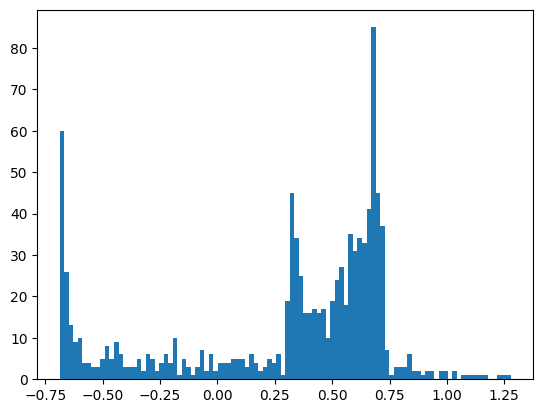
\includegraphics[scale = 0.5]{original data hist.png}
    \caption{Histogram of training data}
    \label{fig:train data hist}
\end{figure}
The plot of the data is given in Fig.\fbox{ \ref{fig:train data}}

\subsubsection{BNN Architecture}

The BNN is designed to have 2 hidden layers, each with 20 neurons. The prior on the weights and biases of each neuron at all layer is $\mathcal{N}(0,1)$. The $\sigma_n ^2$ (standard deviation on the posterior of $y$, $p(y|x, \omega)$) from Eq.\fbox{\ref{eq:1}} is set to random, i.e., $\sigma_n ^2$ $\sim$ $\mathcal{U}(0,1)$. 
Therefore,

\begin{math}
    y|x, \mathcal{D} \sim \mathcal{N}( NN_{\omega}(x), \sigma_n ^2 ) \\ 
    \sigma_n ^2 \sim \mathcal{U}(0,1) \\
    \omega_j \sim \mathcal{N}(0,1) 
\end{math} \\
ADAM optimizer is used and the model is run for 25000 epochs while minimizing the loss function ( a trace implementation of the minimization of ELBO). The parameters of the ADAM optimizer are set to be:

\begin{itemize}
    \item learning rate: 0.001
    \item $\beta_1$: 0.999
    \item $\beta_2$: 0.999
    \item clipping normal: 2.0
\end{itemize}

To check the predictions (both interpolation and extrapolation are performed simultaneously), 500 samples are taken from the VI posterior approximate. 3000 points are in the range $x^{\star} = [-0.5,1.5]$ are predicted on the trained BNN, and the predictions are given in Fig.\fbox{\ref{fig:svi preds}}. The loss function of the SVI training epochs is given in Fig.\fbox{\ref{fig:svi loss function}}.

\begin{figure}[h!]
    \centering
    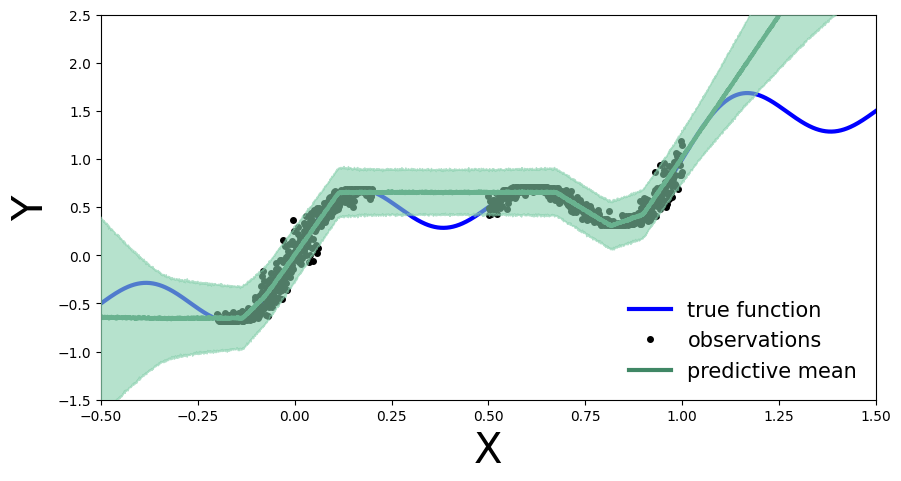
\includegraphics[scale=0.5]{svi preds.png}
    \caption{SVI Predictions}
    \label{fig:svi preds}
\end{figure}


\begin{figure}[h!]
    \centering
    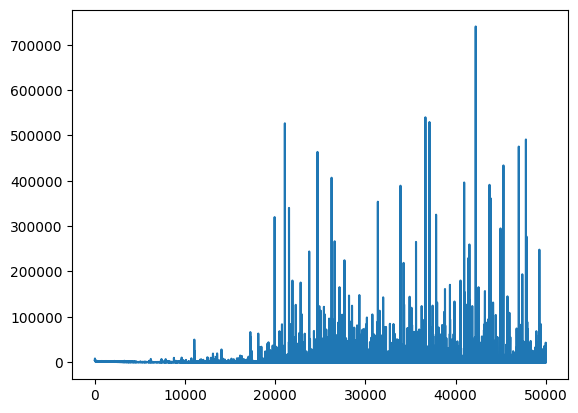
\includegraphics[scale=0.5]{svi loss.png}
    \caption{SVI loss function}
    \label{fig:svi loss function}
\end{figure}

It can observed that the predictions in the interpolated regions perform fairly well. But in the extrapolated regions, $\{[-0.25,-0.5] \cup [0.5,1.0]\}$, the prediction performance is poor. 


\subsection{HMC (No U-Turn Sampler)}
As mentioned before, MCMC can be used to sample from the posterior $p(y,x|\mathcal{D})$. We can use MCMC sampler to get an unbiased estimate of $p(y,x|\mathcal{D})$. \\
\begin{equation}
    p(y,x|\mathcal{D}) = \mathbb{E}_{ \omega \sim p(\omega|\mathcal{D}) }[ p(y|x, \omega) ]
\end{equation}
We can approximate $\mathbb{E}_{ \omega \sim p(\omega|\mathcal{D}) }[ p(y|x, \omega) ]$ through Monte Carlo sampling as

\begin{equation}
    \mathbb{E}_{ \omega \sim p(\omega|\mathcal{D}) }[ p(y|x, \omega) ] \approx \frac{1}{N} \sum_{i=1}^{N} p(y|x, \omega_i)
\end{equation}
where, $\omega_i \sim p(\omega_i| \mathcal{D})$. From Bayes theorem, \\

\begin{equation}
    p(\omega|\mathcal{D}) = \frac{p(\mathcal{D}|\omega) p(\omega)}{p(\mathcal{D})}
\end{equation} \\
So, $\omega_i \sim p(\omega_i| \mathcal{D}) \propto p(\mathcal{D}|\omega) p(\omega) $ are drawn from the posterior distribution. Because the normalizing constant is intractable, we require MCMC methods like Hamiltonian Monte Carlo to draw samples from the non-normalized posterior. Specifically, the No U-Turn Sampler (NUTS), a variant of the HMC sampler is used to sample from the posterior. The number of steps taken by the integrator is dynamically adjusted on each sample to ensure an optimal length for the Hamiltonian trajectory. As such, the samples generated will typically have lower autocorrelation than those generated by the HMC. \\
HMC’s performance depends strongly on the tuning parameters $M$ (momentum covariance/ mass matrix), $\epsilon$ (step size in chain), and $L$ (number of steps per iteration/ length of chain).
NUTS is an extension of HMC that adaptively tunes $M$ and $\epsilon$ during burn-in, and adapts $L$ throughout the MCMC run. NUTS eliminates the need to select the tuning parameters. The basic idea of NUTS is that the MC propagates the Hamiltonian dynamics until the trajectory starts going back towards where it started. The intuition is that we want to make as big a move as possible, so going back toward where we started is undesirable. NUTS is a way of constructing trajectories to avoid going back (momentum vector pointing in the direction of initial position), while still satisfying detailed balance.
This is implemented via a procedure for choosing $L$ adaptively. NUTS also employs a method of adapting $\epsilon$ and $M$ during the burn-in period. \\

In addition, the vanilla HMC algorithm is used to sample from the posterior. The parameters of the HMC sampler are:
\begin{itemize}
    \item $\epsilon$ = 0.0001
    \item $L$ = 5
\end{itemize} \\
The HMC is run to sample from the posterior, with the BNN trained on $\{x_{train}, y_{train}\}$ as the potential function, and the results are plotted in Fig.\fbox{\ref{fig:vanilla hmc}}

\begin{figure}[h!]
    \centering
    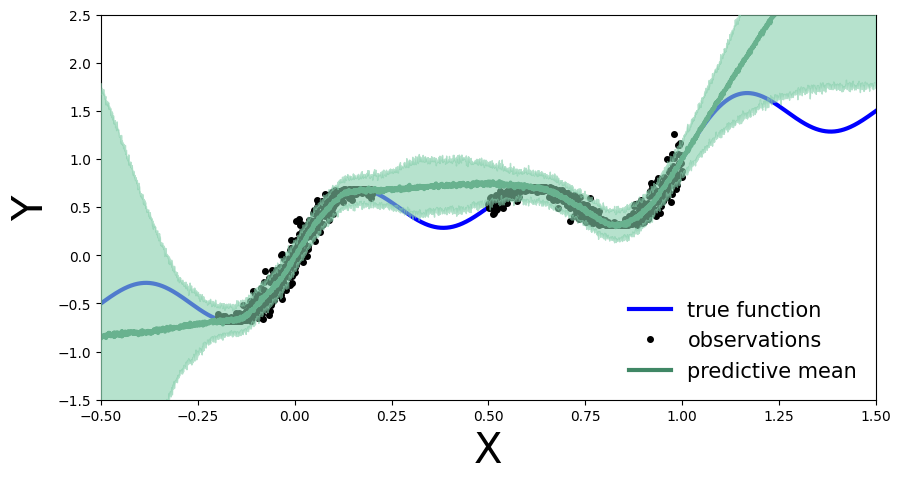
\includegraphics[scale=0.5]{vanilla hmc.png}
    \caption{Vanilla HMC sampler for BNN}
    \label{fig:vanilla hmc}
\end{figure}
The potential function for the NUTS sampler is the neural network and 550 samples from the posterior are sampled, with a burn in of 50 samples. The parameters of the HMC chains are adaptive and don't need to be specified explicitly. The predictions and the uncertainty is plotted in Fig.\fbox{\ref{fig:nuts}}.
\begin{figure}[h!]
    \centering
    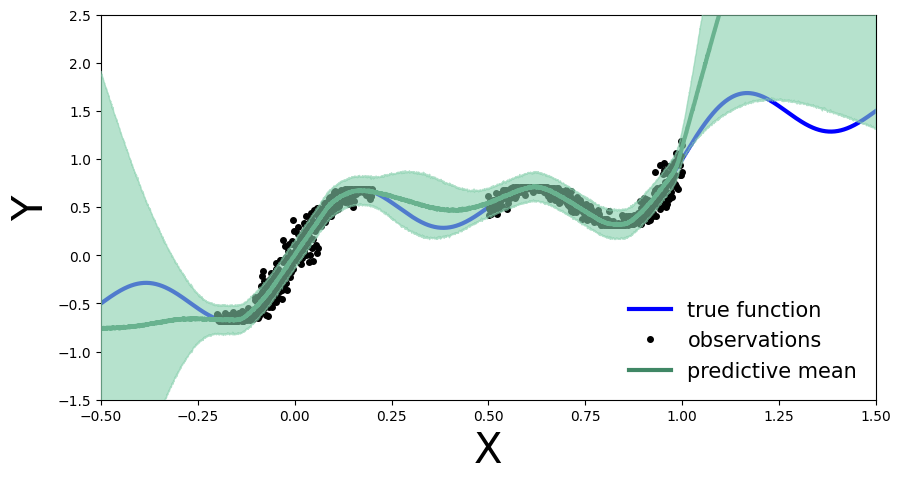
\includegraphics[scale=0.5]{nuts.png}
    \caption{NUTS Sampler for BNN}
    \label{fig:nuts}
\end{figure}

\subsubsection{Comparing posteriors}
Inspecting the posteriors of the weights of all neurons in the first hidden layer (20 distributions), a plot of the posteriors from SVI and NUTS are compared in Fig.\fbox{\ref{fig:posteriors}}.

\begin{figure}[h!]
    \centering
    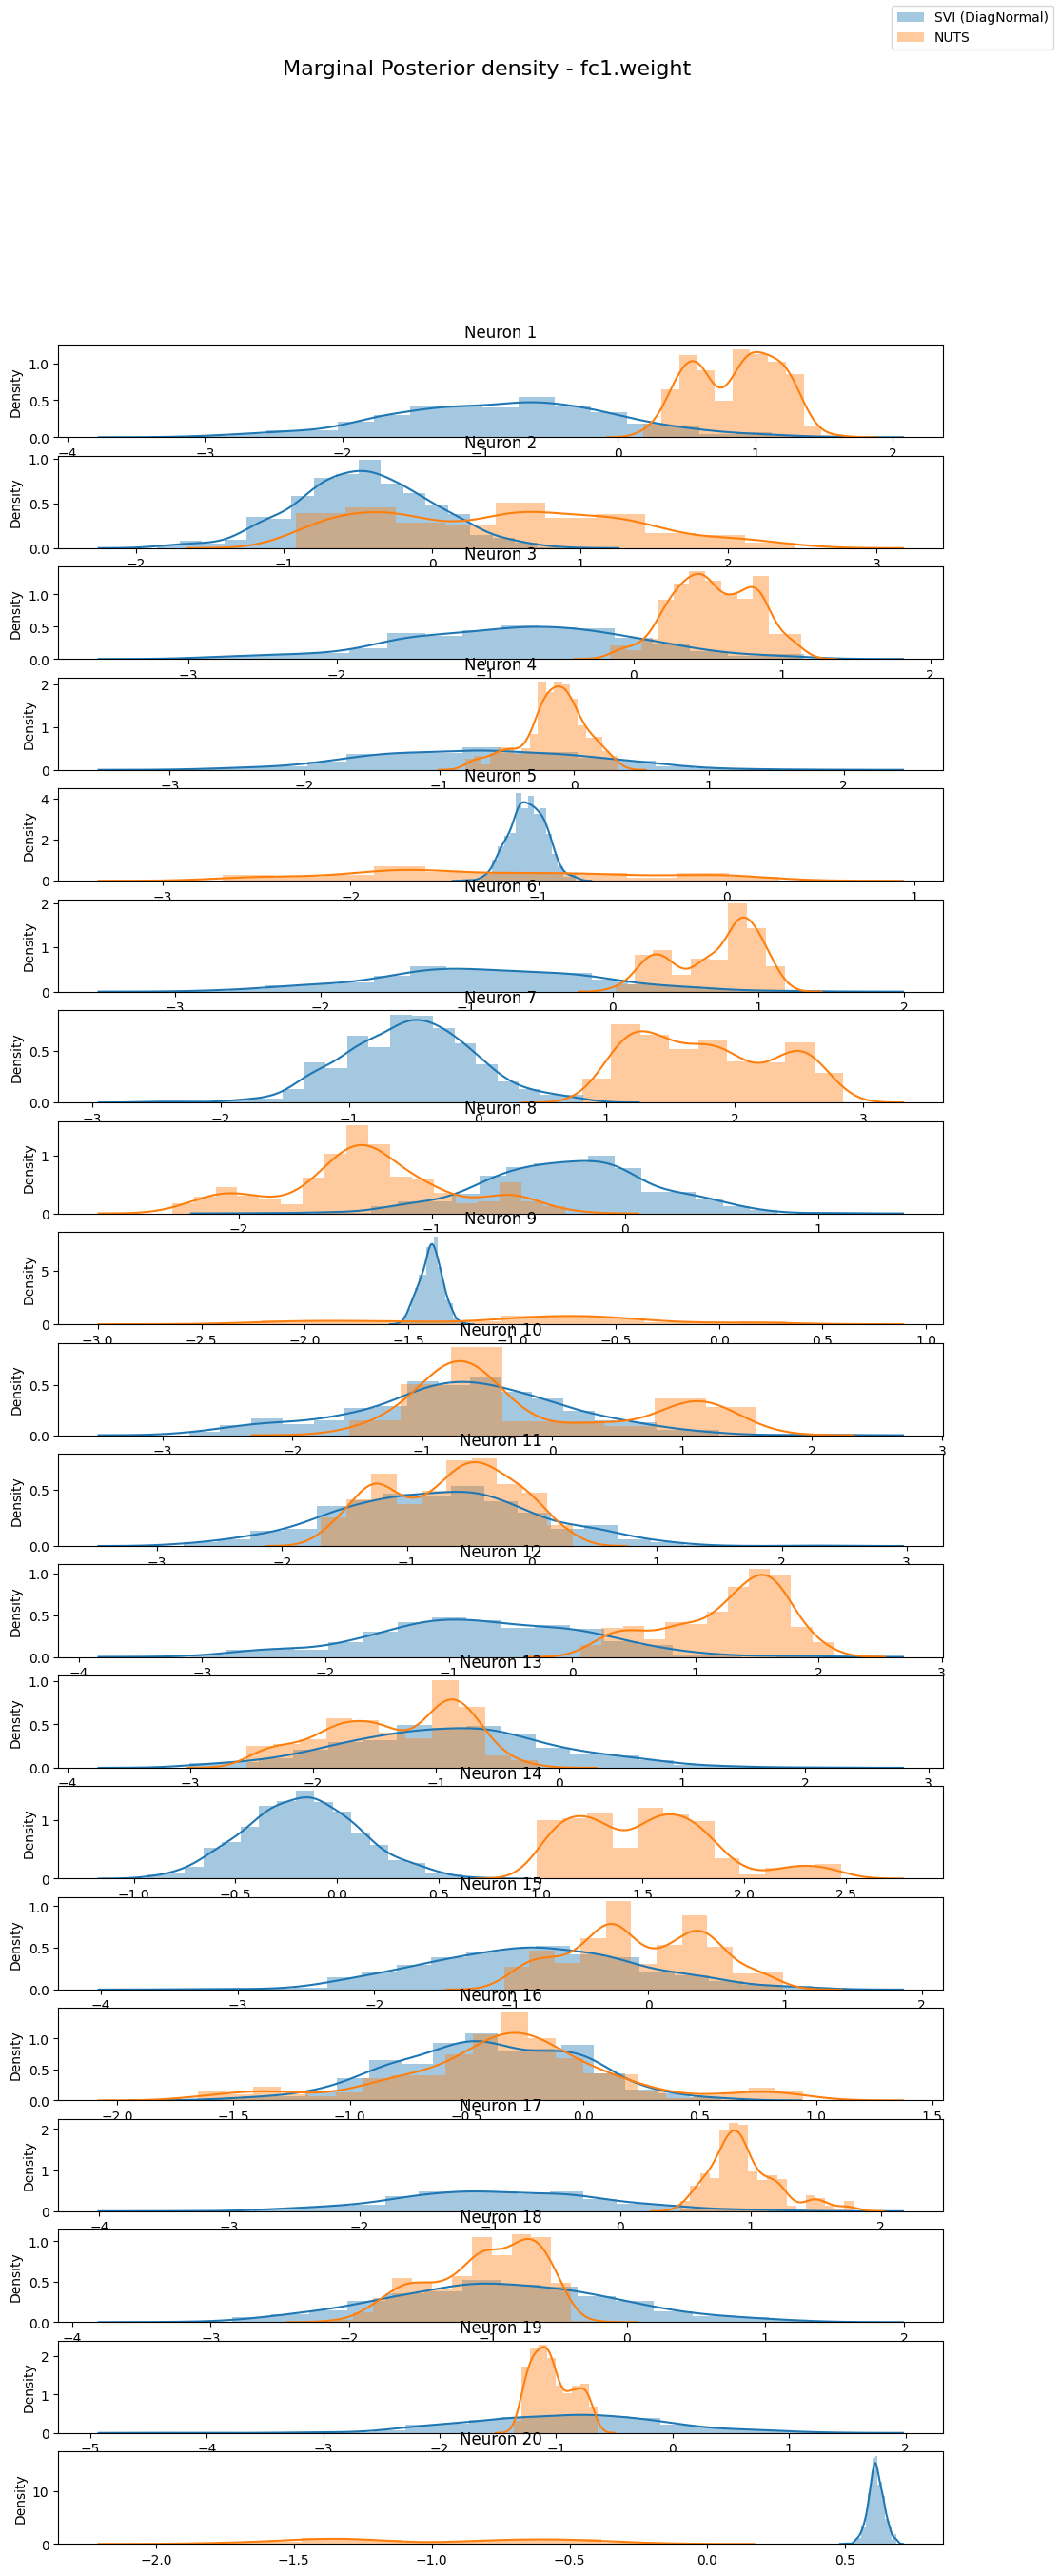
\includegraphics[scale=0.25]{posteriors.png}
    \caption{Posteriors of SVI vs NUTS}
    \label{fig:posteriors}
\end{figure}

\subsection{Deterministic NN}
To compare the BNN with deterministic NN, a point estimate of the NN (MAP estimate) is created using a fully connected MLP. The prediction of the single NN is plotted in Fig.\fbox{\ref{fig:one nn}}.
% A small study is conducted to check for the best architecture to train the deterministic NN. With a fixed number of hidden layers (2 layers), the NN is trained on multiple architectures with varying numbers of neurons per layer (10,20,30,40).

% \begin{figure}
%     \centering[h!]
%     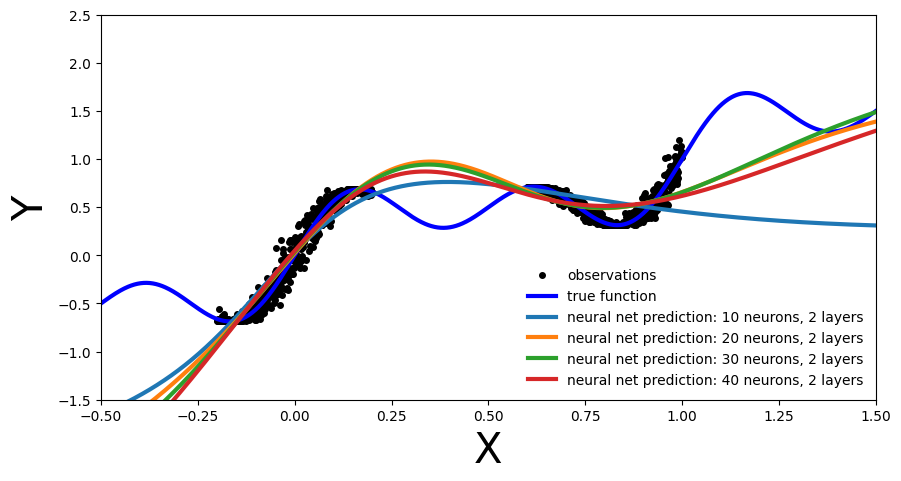
\includegraphics[scale=0.5]{deterministic nn comparision.png}
%     \caption{Comparison of multiple architectures}
%     \label{fig:comparison det nn }
% \end{figure}
% From \fbox{\ref{fig:comparison det nn }} it seems like the initial assumption of the architecture (2 hidden layers with 20 neurons each) fits the data well.

\begin{figure}[h!]
    \centering
    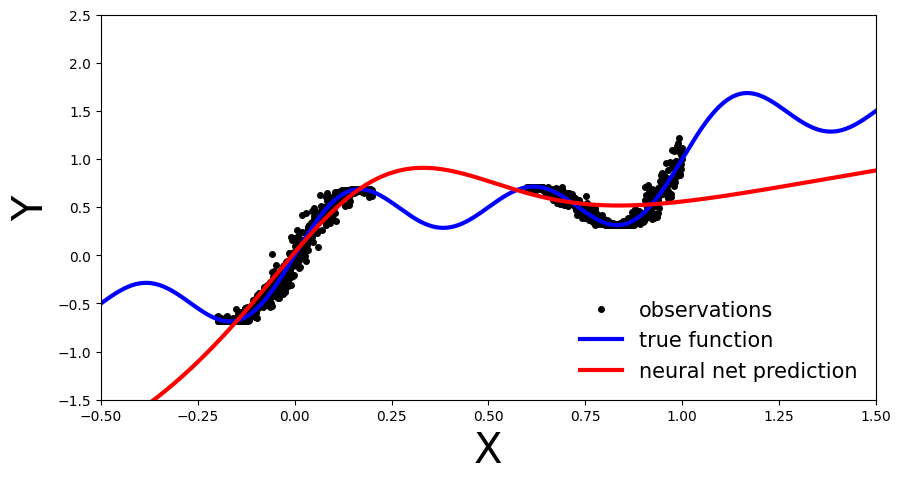
\includegraphics[scale=0.5]{deterministic nn.png}
    \caption{Neural Network with 2 layers, 20 neurons each}
    \label{fig:one nn}
\end{figure}


\subsection{Deep Ensemble}
In deep ensemble, multiple point estimates of the NN are trained and the final prediction is computed as an average across the models. From a Bayesian perspective, the different point estimates correspond to samples of a Bayesian posterior. This can be interpreted as approximating the posterior with a distribution parametrized as multiple Dirac deltas.

\begin{equation}
    q_{\phi}(\omega|\mathcal{D}) = \sum_{\omega_i} \alpha_{\omega_i}\delta_{\omega_i}(\omega)
\end{equation}
where $\alpha_{\omega_i}$  are positive constants such that their sum is equal to one.
It is assumed that $\alpha_{\omega_i} = 1/N_{ensemble}$ for all the networks in the ensemble. 10 networks are considered to be an ensemble. The ensemble's predictive functions are plotted in Fig.\fbox{\ref{fig:ensemble}}.

\begin{figure}[h!]
    \centering
    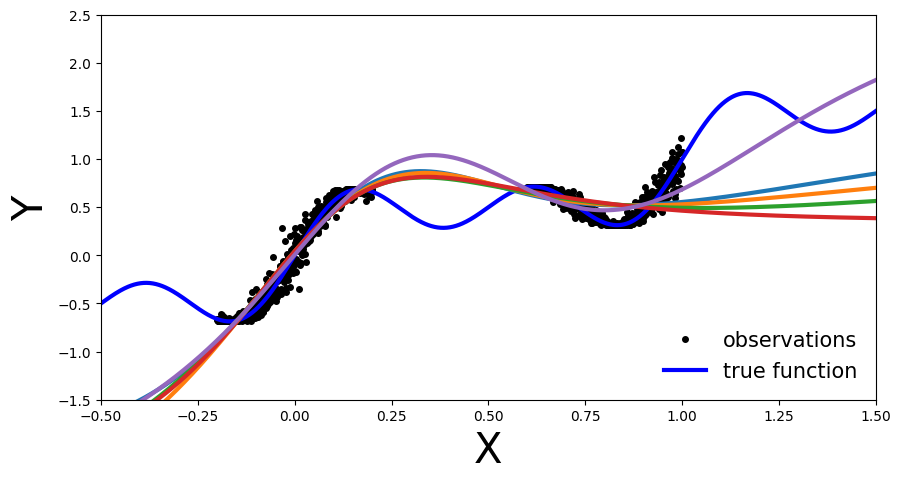
\includegraphics[scale=0.5]{ensemble.png}
    \caption{Ensemble}
    \label{fig:ensemble}
\end{figure}
The uncertainty bands of the ensemble NN is plotted in \fbox{\ref{fig:ensemble uncertainty}}

\begin{figure}[h!]
    \centering
    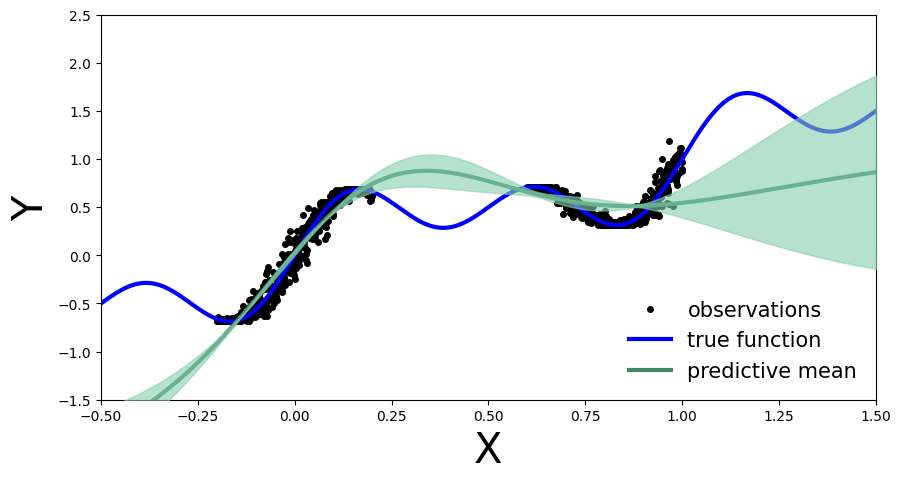
\includegraphics[scale=0.5]{ensemble uncertainty.png}
    \caption{Uncertainty bands of ensemble NN}
    \label{fig:ensemble uncertainty}
\end{figure}


\subsection{Gaussian Process Regression}

Gaussian Process Regression is trained to quantify the epistemic uncertainty. The mathematics of the GPR with noisy data is adapted from the class notes. The GP is assumed to have an RBF kernel with $length-scale=0.05$ and $variance = 0.02$ (initial parameters). The optimum hyperparameters for the GP are obtained by optimizing the maximum likelihood function using L-BFGS optimizer. The GP before maximum likelihood estimation on the training data is plotted in Fig.\fbox{\ref{fig:crude gpr}}.
\begin{figure}[h!]
    \centering
    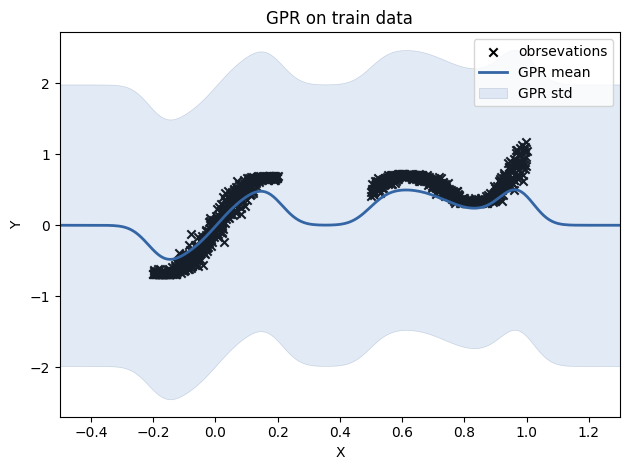
\includegraphics[scale=0.5]{gpr unoptimized.png}
    \caption{GPR without optimizing hyperparameters}
    \label{fig:crude gpr}
\end{figure}
The performance of the GPR on the training data is plotted in Fig.\fbox{\ref{fig:gpr mle train}}.
\begin{figure}
    \centering[h!]
    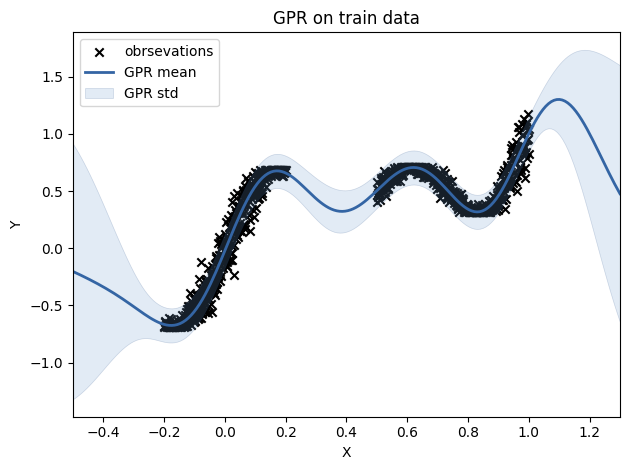
\includegraphics[scale=0.5]{gpr train.png}
    \caption{GPR with optimized hyperparameters on training data}
    \label{fig:gpr mle train}
\end{figure}
The performance of the GPR on the test data, $x_{\text{test}} = [-0.5,1.5]$ is shown in Fig.\fbox{\ref{fig:gpr mle test}}

\begin{figure}[h!]
    \centering
    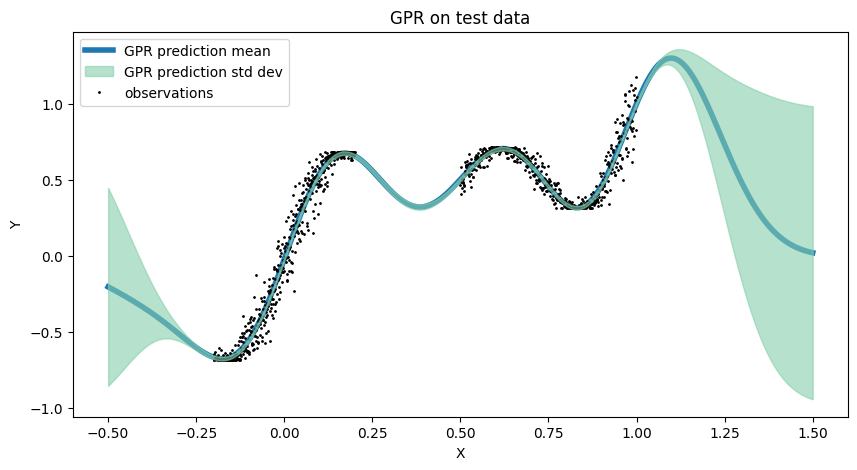
\includegraphics[scale=0.5]{gpr test.png}
    \caption{GPR with MLE on test data}
    \label{fig:gpr mle test}
\end{figure}

\section{Conclusions}

\begin{itemize}
    \item \textbf{SVI:} The SVI does not capture the interpolation and extrapolation predictions very well. The training data is chosen such that the gradients at the beginning and end of the data are close to 0. Hence, the gradient update at the ends of the dataset remains  in the same direction as that of the last points. Hence, the interpolation and extrapolation standard deviations are high. This behavior does not seem to improve with an increase in training epochs.
    As SVI is an approximation of the posterior, we used a normal distribution with a learnable mean and a diagonal covariance matrix. It is clear that for this specific example, this method leads to a very poor approximation of the actual posterior since it can only fit an unimodal distribution. This highlights the major limitations of simple VI methods for BNNs.
    \item \textbf{HMC:} The HMC sampler was used to generate samples from the posterior. It is observed that HMC has a lesser probability of acceptance (70\%) compared to that of NUTS (91\%). The posterior samples of HMC have high variance and hence the boundaries of the standard deviation and mean are jagged compared to NUTS sampler. Vanilla HMC is very difficult to adapt and takes a very long time to train even for the small dataset.
    \item \textbf{NUTS:} The NUTS sampler was used mainly as a way of generating samples from the true posterior. The MCMC sampler provides a very good approximation of samples from the exact posterior. The NUTS sampler for BNN posterior captures the interpolation better than the SVI model does. The uncertainty, as measured by the standard deviation a posteriori, is low where the data points lie and increases with distance away from the observations.
    \item \textbf{Deterministic NN:} The deterministic neural network gives only prediction and no information about the uncertainty.
    \item \textbf{Deep Ensemble:} Ensembling is the most straightforward way to perform ensemble learning with an NN and is done by just restarting the learning procedure multiple times. Using this strategy to learn the posterior gives quite good results, even better than naive VI as the samples can belong to different modes of the posterior. The main drawback of this approach is that it provides no estimation of the local uncertainty around the different modes of the posterior.
    \item \textbf{Gaussian Process Regression:} GPR has a nice mechanism for incorporating prior beliefs about the underlying function by specifying mean and covariance functions. This trains well compared to BNNs where training depends on a lot of hyperparameters and requires fine tuning. In BNNs, it is difficult to incorporate intuitive prior information about the functions. Rather, in BNNs priors over the network parameters are specified and are interpreted as a bias towards less complex functions (posterior) via smaller weights (generally normal distributions). For this particular small-scale example, GP performs significantly better in predicting the data in  both interpolation and extrapolation. The variance at the points where observations are present is less and the mean of the GPR prediction fits the true mixture of sines best compared to the BNNs. However, Gaussian Processes have scalability limitations making BNNs a more practical model in large data settings, although this has not been demonstrated in this work.
    
\end{itemize}

\begin{thebibliography}{9}
\bibitem{hoffman}
https://jmlr.org/papers/volume14/hoffman13a/hoffman13a.pdf

\bibitem{jones}
https://andrewcharlesjones.github.io/journal/svi.html

\bibitem{audrey}
Olivier, A., Shields, M.D. and Graham-Brady, L., 2021. Bayesian neural networks for uncertainty quantification in data-driven materials modeling. Computer methods in applied mechanics and engineering, 386, p.114079.

\bibitem{jospin}
Jospin, L.V., Laga, H., Boussaid, F., Buntine, W. and Bennamoun, M., 2022. Hands-on Bayesian neural networks—A tutorial for deep learning users. IEEE Computational Intelligence Magazine, 17(2), pp.29-48.
\end{thebibliography}

\end{document}
